\documentclass[hyperref=colorlinks]{beamer}
\mode<presentation>
\usetheme{iclpt}
\setbeamertemplate{navigation symbols}{}
\setbeamertemplate{headline}{
  \begin{beamercolorbox}[leftskip=.2cm,rightskip=.2cm,topskip=.2cm,ht=1.1cm,dp=0.1cm,wd=\textwidth]{institute in head/foot}
    
\includegraphics[height=1cm]{icl.pdf}
    \hfill
%    \includegraphics[height=1cm]{../Pics/ATLAS-Logo-Square-Blue-RGB.png}
%    
\includegraphics[height=1cm]{../Pics/CMS-Color.pdf}
    
\includegraphics[height=1cm]{TalkPics/t2k_logo_large.png}

%??put t2k logo here
  \end{beamercolorbox}
}
\setbeamertemplate{footline}{
  \begin{beamercolorbox}[ht=.35cm,dp=0.2cm,wd=\textwidth,leftskip=.3cm]{author in head/foot}%
    \begin{minipage}[c]{5cm}%
      \usebeamerfont{author in head/foot}
      \insertshortauthor 
      \insertshorttitle
    \end{minipage}\hfill%
    \hfill
    \insertframenumber{} / \ref{lastframe}
    %\hfill
    \begin{minipage}{6cm}
      \hfill
      %\insertshorttitle
    \end{minipage}
  \end{beamercolorbox}%
}

\definecolor{beamer@icdarkblue}{RGB}{0,51,102}
\definecolor{beamer@icmiddleblue}{RGB}{0,82,150} 
\definecolor{beamer@iclightblue}{RGB}{200,212,232}
\definecolor{beamer@icmiddlered}{RGB}{204,51,0}
\definecolor{beamer@iclightred}{RGB}{232,212,32}

\usepackage{tikz}
\usetikzlibrary{arrows,shapes,backgrounds}
\usepackage{color}
\usepackage{tabularx,colortbl}
\usepackage{graphicx}
\usepackage{pdfpages}
\usepackage{feynmp}
\usepackage{rotating}
\usepackage{moresize}
\usepackage{slashed}
\usepackage{xcolor,colortbl}
\DeclareGraphicsRule{*}{mps}{*}{}
\hypersetup{colorlinks=false}

\title[2D vs 1D yields]{\vspace{-0.2cm} 2D vs 1D yields}
\author[P. Dunne]{Patrick Dunne - Imperial College London}
\titlegraphic{
  \vspace{-0.4cm}
}
\date{}
\begin{document}
\tikzstyle{every picture}+=[remember picture]
\tikzstyle{na} = [baseline=-.5ex]
\begin{fmffile}{t2ktemplatefeyndiags}


  %TITLE PAGE
  %20 mins + 5 questions
  \section{Title}
  \begin{frame}
    \titlepage
  \end{frame}

  \begin{frame}
    \frametitle{Overview}
    \begin{block}{}
      \begin{itemize}
      \item Previously checked 2D vs 1D yields from SK\_plots2015
      \item[-] Agreement was good for all ``styles'' with only small CCQE differences
      \item After modifications to make jointfit code work with 2D splines I compared my kinematic plots to those from VALOR
      \item Saw differences in some bins and whilst investigating this I found that my 1D and 2D rates no longer agree
      \item Have checked 1D version against MaCh3 note and see good but not perfect agreement
      \item[-] 1D MaCh3 rates agree with 2D VALOR rates to less than 1\%
      \end{itemize}
    \end{block}
  \end{frame}

  \begin{frame}
    \frametitle{Current situation}
    \begin{block}{}
      \begin{itemize}
        \item Rates from styles 0 and 1 agree
        \item Style 2 has differences for nue sample in CCQE, CC1pi, CCCoh (osc only), NCPi0, NCPi+- and 2p-2h (osc only)
        \item Have isolated difference to xsec\_w\_1 weight in samplePDFNue, leads to $\sim$10\% differences
      \end{itemize}
    \end{block}
  \end{frame}

  \begin{frame}
    \frametitle{2D Markov Chain}
    \begin{block}{}
      \begin{itemize}
      \item Also ran 1M event chain using GPU machine at IC
      \item[-] Able to run 2 jobs at a time (just)
      \item Took $\sim$3 days
      \item Caveat that above differences might affect the results
      \end{itemize}
    \end{block}
  \end{frame}

  \begin{frame}
    \frametitle{1M step chain contour - appearance}
    \centering
    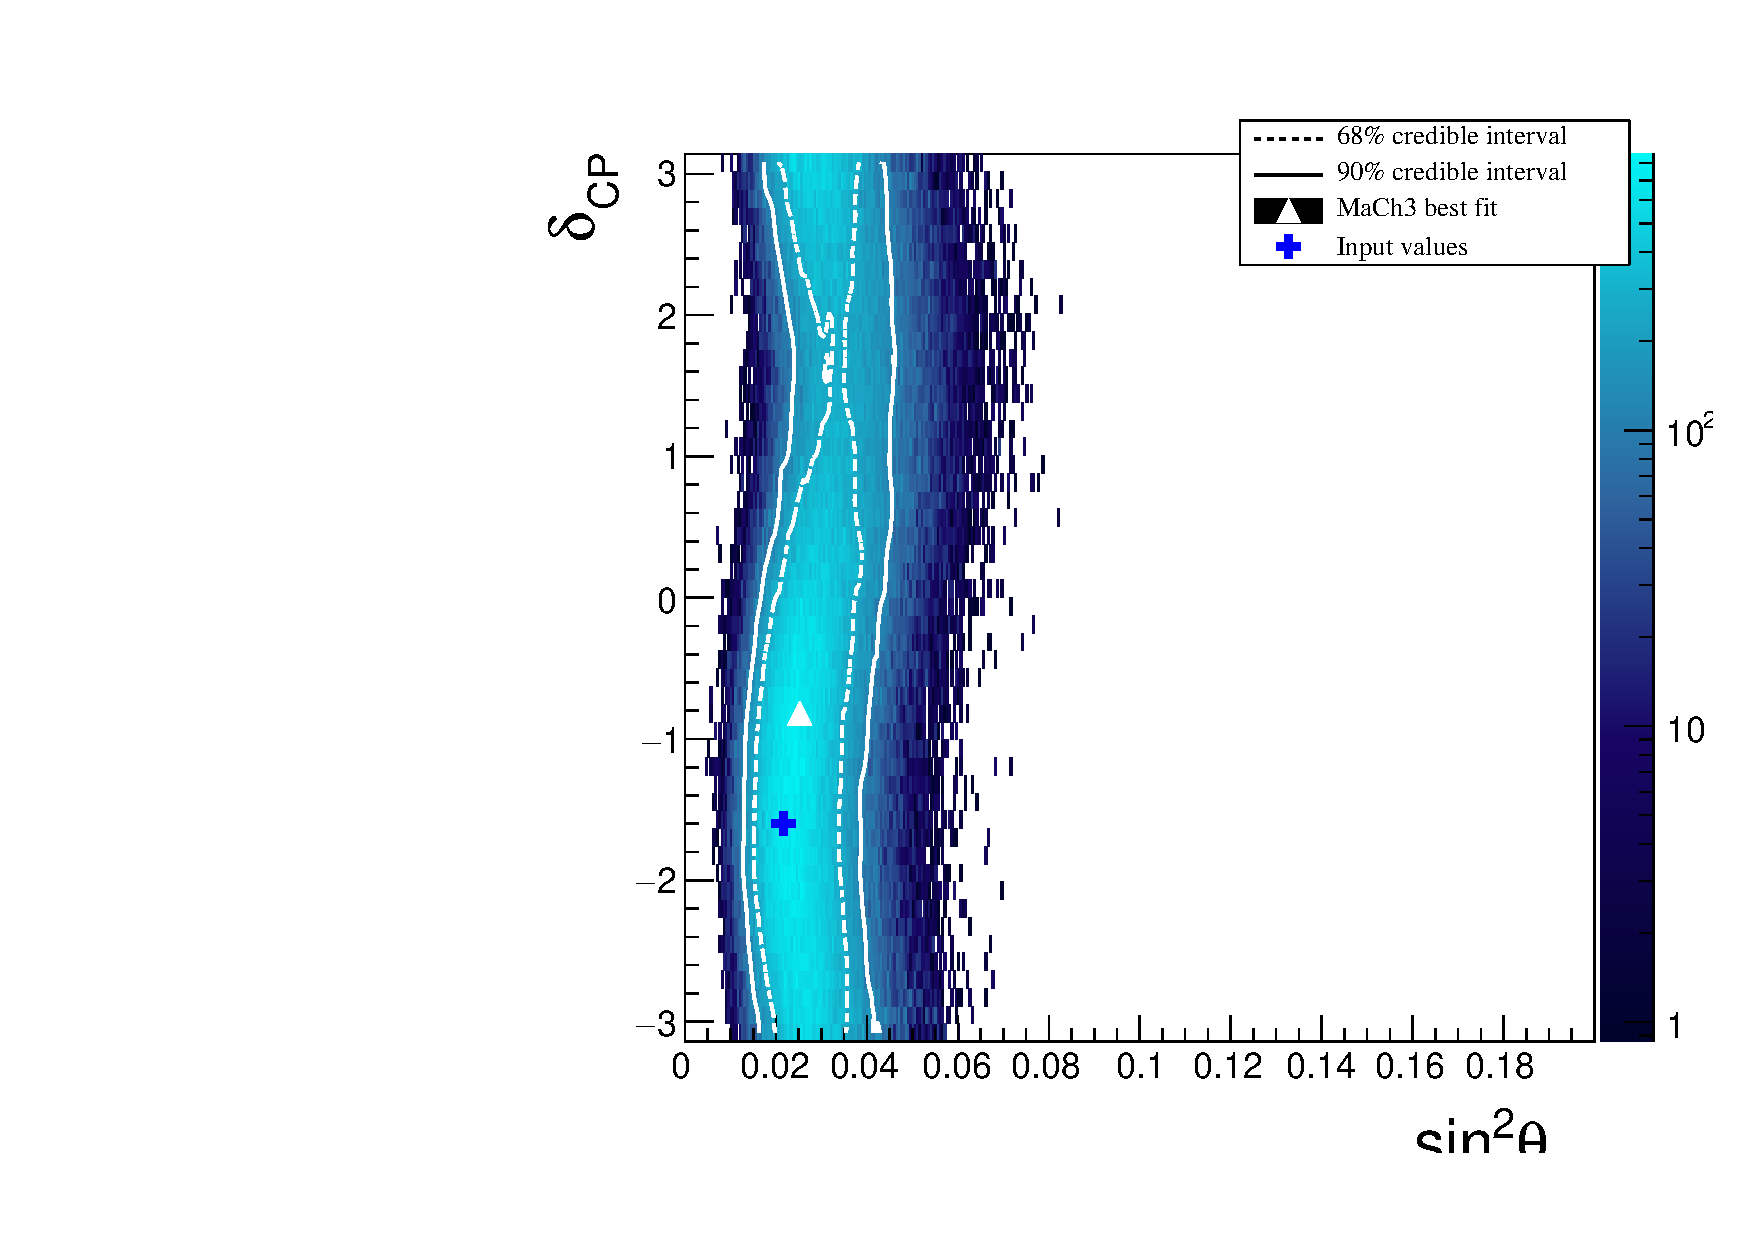
\includegraphics[width=.65\textwidth]{TalkPics/2dvs1dyields_100516/contours_appearance_graph.pdf}
  \end{frame}

  \begin{frame}
    \frametitle{1M step chain contour - disappearance}
    \centering
    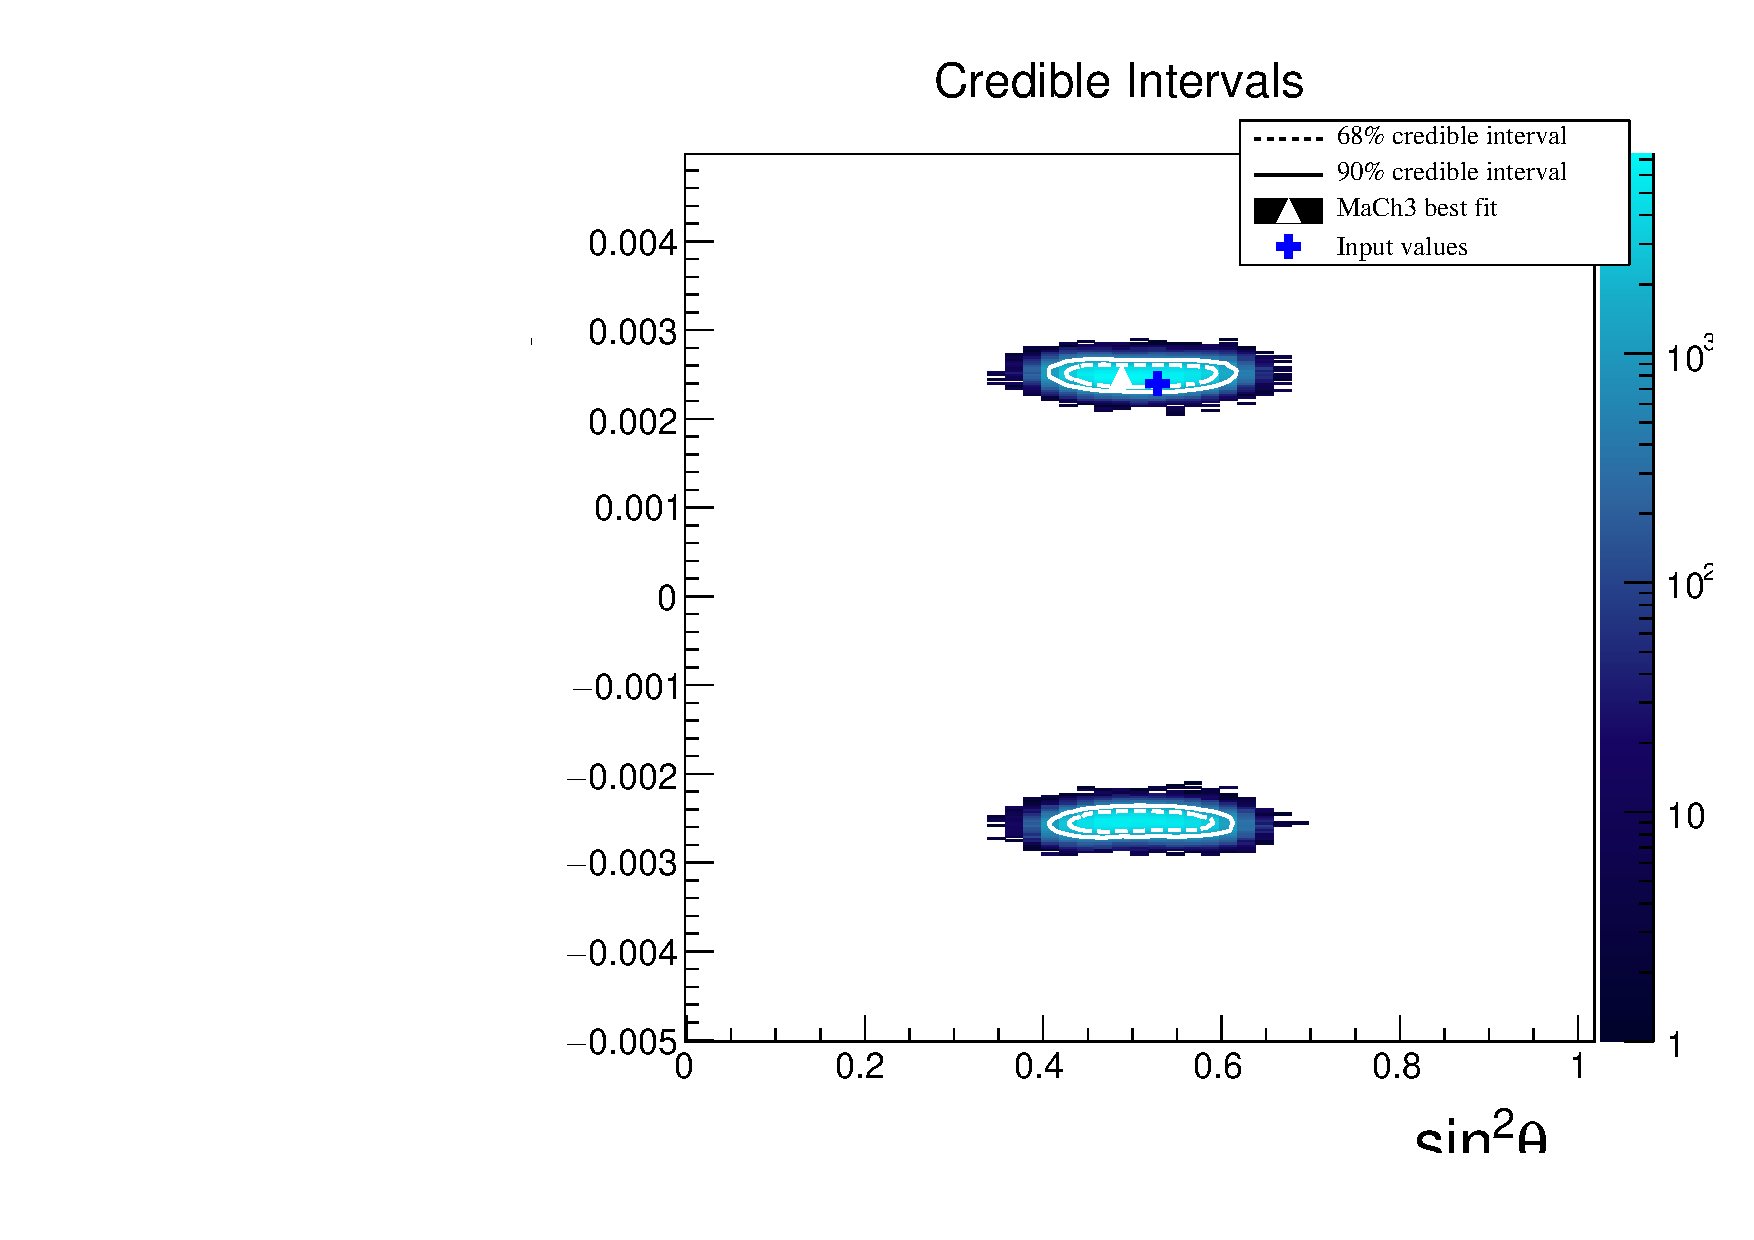
\includegraphics[width=.65\textwidth]{TalkPics/2dvs1dyields_100516/contours_disappearance_graph.pdf}
  \end{frame}


  \begin{frame}
    \frametitle{}
    \label{lastframe}
    \begin{block}{}
      \begin{itemize}
      \item Can run chains in 2D
      \item 2D vs 1D rate differences being investigated
      \item Agreement with VALOR good in most bins
      \item[-] 2 bins do see significant difference
      \end{itemize}
    \end{block}
  \end{frame}

  %Backup goes here
  
\end{fmffile}
\end{document}

